\documentclass{standalone}
\usepackage{tikz}
\usepackage{pgfplots}
\pgfplotsset{compat=1.18}
\begin{document}
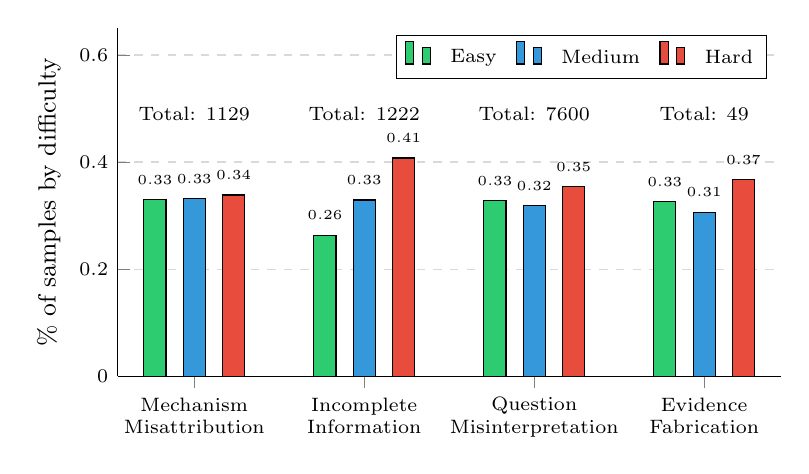
\begin{tikzpicture}[font=\small]
    % Define common colors
    \definecolor{easycolor}{RGB}{46,204,113}
    \definecolor{mediumcolor}{RGB}{52,152,219}
    \definecolor{hardcolor}{RGB}{231,76,60}
    
    \begin{axis}[
        width=10cm,
        height=6cm,
        ybar,
        bar width=8pt,
        ymin=0, ymax=0.65,
        ylabel={\% of samples by difficulty},
        symbolic x coords={MPM, II, MQ, MEF},
        xtick=data,
        xticklabels={
            {Mechanism\\Misattribution},
            {Incomplete\\Information},
            {Question\\Misinterpretation},
            {Evidence\\Fabrication}
        },
        x tick label style={align=center, font=\scriptsize},
        y tick label style={font=\scriptsize},
        legend style={
            at={(0.98,0.98)},
            anchor=north east,
            font=\scriptsize,
            legend columns=-1,
            transpose legend,
            row sep=0pt,
            column sep=5pt
        },
        ymajorgrids=true,
        grid style={dashed, gray!30},
        nodes near coords,
        every node near coord/.append style={
            anchor=south,
            font=\tiny,
            yshift=2pt
        },
        enlarge x limits=0.15,
        axis lines*=left  % This is the key change - only shows left axes
    ]
        \addplot[fill=easycolor, bar shift=-0.5cm] coordinates {
            (MPM, 0.3295) (II, 0.2635) (MQ, 0.3276) (MEF, 0.3265)
        };
        \addplot[fill=mediumcolor, bar shift= 0.00cm] coordinates {
            (MPM, 0.3322) (II, 0.3290) (MQ, 0.3182) (MEF, 0.3061)
        };
        \addplot[fill=hardcolor, bar shift= 0.5cm] coordinates {
            (MPM, 0.3384) (II, 0.4075) (MQ, 0.3542) (MEF, 0.3673)
        };
        \legend{Easy, Medium, Hard}
        
        \node[anchor=south] at (axis cs: MPM, 0.46) {\scriptsize Total: 1129};
        \node[anchor=south] at (axis cs: II, 0.46) {\scriptsize Total: 1222};
        \node[anchor=south] at (axis cs: MQ, 0.46) {\scriptsize Total: 7600};
        \node[anchor=south] at (axis cs: MEF, 0.46) {\scriptsize Total: 49};
        
    \end{axis}
\end{tikzpicture}
\end{document}